\newcommand*{\StatePattern}{\begingroup

%----------------------------------------------------------------------------------------
%	State Pattern
%----------------------------------------------------------------------------------------
\chapter{State Pattern}
As mentioned in chapter \ref{ch:embeddedReactiveSystems}, a characteristic of a reactive system is that responses of the reactive system are dependent on the current state of the system. Usually an embedded reactive system is able to change its state. A simple example of this is a system with a failure state. If everything meets the expectations, the system stays in its normal state. But if something unexpected occurs, the system switches to its failure state. Within the failure state the system tries to keep the essential subsystems running and minimizes the damages within the environment. Other stateful systems like a remote control extend the functionality of the system with a limited number of buttons. Depending on the state, the remote control is able to communicate with either the television, dvd player or another multimedia device. 

\begin{floatingfigure}[rh]{72mm}
\centering
\mbox{\frame{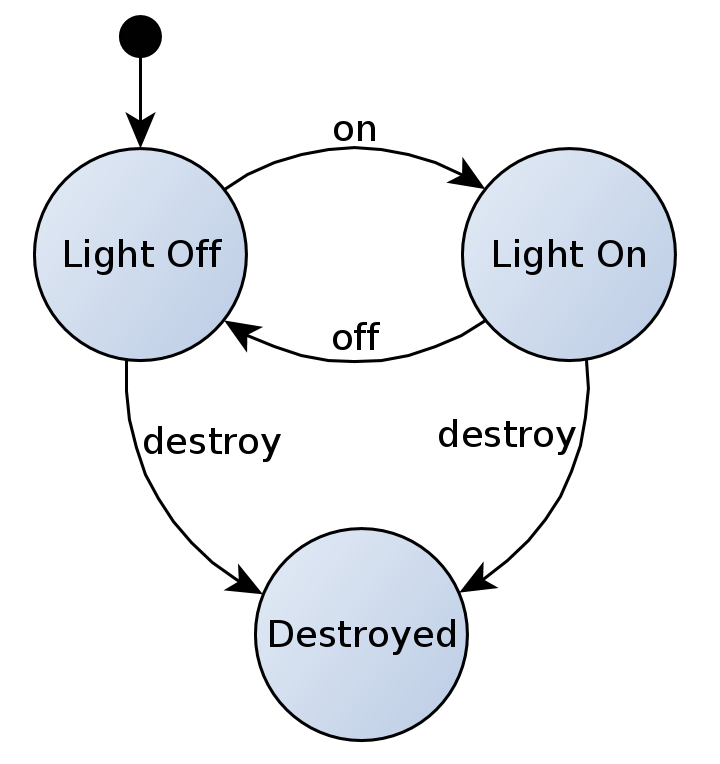
\includegraphics[width=70mm]{Images/StateMachineLight.png}}}
\caption{State machine of a light.}
\label{fig:stateMachineLight}
\end{floatingfigure}

\noindent Figure \ref{fig:stateMachineLight} shows a simple example of a state machine with three states and three signals. \emph{Light Off} is the initial state. The system can change to the state \emph{Light On} by the signal 'on' and to the state \emph{Destroyed} by the signal 'destroy'. From state \emph{Line On} the system can change back to the state \emph{Light Off} or to the state \emph{Destroyed}. \emph{Destroyed} is a final state. When the light is destroyed, it is destroyed. \\

\noindent The state pattern is an object based pattern of the type behavioral. The problem is how to react depending on the current state and the external stimuli with a minimum of overhead in timing. Procedural implementations solve this problem by providing a matrix where the combination of the current state and the input determine behavior and the transition to the next state. Other implementations work with a number of switch-case-selections. The result of these implementations is difficult read and to maintain. The base of the state pattern of GoF is a context class and an abstract base state class. (Figure \ref{fig:statePattern}) Concrete states derive from the base state class and implement the interface. \emph{Context} is the connection between \emph{Client} and the state machine. It contains an instance of the state machine and provides the same interface as the state machine for delegating the incoming signals. \emph{Client} does only know \emph{Context}. It uses \emph{Context} as if it would be a concrete State class. The state machine has access to public member variables of \emph{Context}. \cite[cf.][372 - 377]{GoF2015} 

\begin{figure}[]{}
\centering
\mbox{\frame{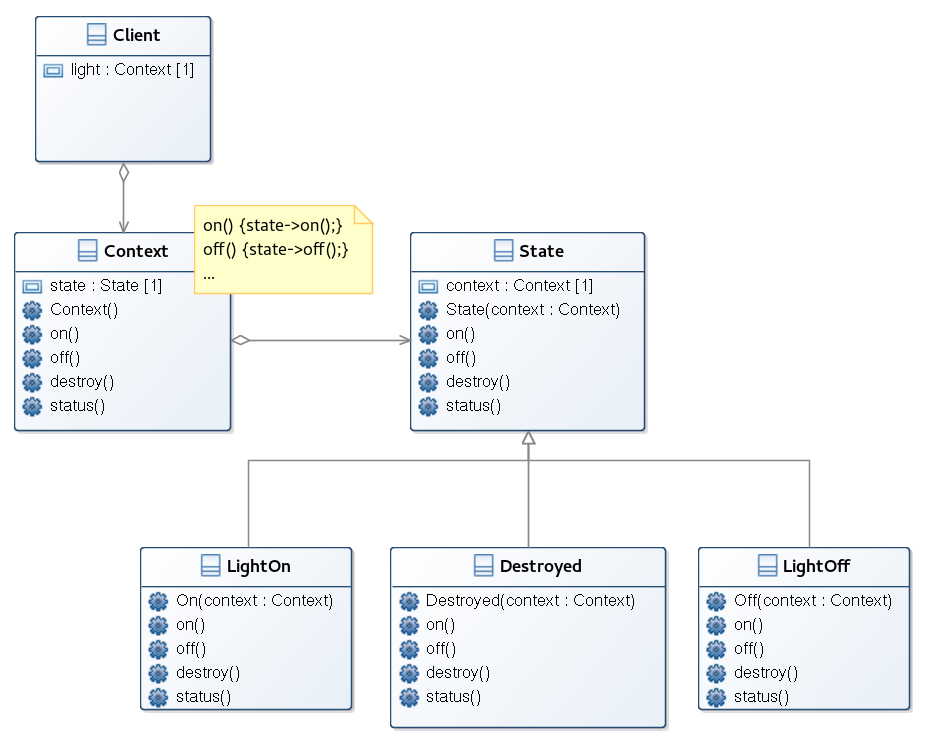
\includegraphics[width=\textwidth]{Images/StatePattern.png}}}
\caption{State pattern UML}
\label{fig:statePattern}
\end{figure}

%----------------------------------------------------------------------------------------
%	Polymophism Implementation
%----------------------------------------------------------------------------------------
\section{Polymophism Implementation}\label{sec:polymophismImplementation}
\noindent The example explained by GoF uses polymorphism. The concrete states use the interface of the abstract base state class (Listing \ref{lst:statePatternAbstractStateCpp03}) and implement the behavior. (Listing \ref{lst:statePatternLightOffDeclarationCpp03} and \ref{lst:statePatternLightOffImplementationCpp03}) \emph{Context} (Listing \ref{lst:statePatternContextCpp03}) contains an instance of \emph{LightOff} as initial state. \emph{Context} and \emph{State} depend on each other. This circular dependency can be solved by forward declaration. Therefore it is necessary to declare \emph{Context} once within the header file of \emph{State} (Listing \ref{lst:statePatternAbstractStateCpp03}, line 1) and include the header file of \emph{Context} later within the implementation of the concrete states. (Listing \ref{lst:statePatternLightOffImplementationCpp03}, line 4) Depending on the behavior of the state machine, similar dependencies occur between concrete states and can be solved on a similar way. \emph{Context} also provides a dispatcher which receives external signals and calls the particular functions. 

\lstinputlisting[caption={State pattern Context C++03}\label{lst:statePatternContextCpp03},captionpos=t, backgroundcolor = \color{white}, frame=single, language=C++, firstline=1, lastline=33]{Sourcecode/StatePattern/ContextCpp03.h}

\FloatBarrier
\lstinputlisting[caption={State pattern abstract State C++03}\label{lst:statePatternAbstractStateCpp03},captionpos=t, backgroundcolor = \color{white}, frame=single, language=C++, firstline=1, lastline=17]{Sourcecode/StatePattern/StateCpp03.h}

\FloatBarrier
\lstinputlisting[caption={State pattern LightOff declaration C++03}\label{lst:statePatternLightOffDeclarationCpp03},captionpos=t, backgroundcolor = \color{white}, frame=single, language=C++, firstline=1, lastline=13]{Sourcecode/StatePattern/LightOffCpp03.h}

\FloatBarrier
\newpage
\lstinputlisting[caption={State pattern LightOff implementation C++03}\label{lst:statePatternLightOffImplementationCpp03},captionpos=t, backgroundcolor = \color{white}, frame=single, language=C++, firstline=1, lastline=22]{Sourcecode/StatePattern/LightOffCpp03.cpp}

\FloatBarrier
\lstinputlisting[caption={State pattern Client C++03}\label{lst:statePatternClientCpp03},captionpos=t, backgroundcolor = \color{white}, frame=single, language=C++, firstline=1, lastline=11]{Sourcecode/StatePattern/ClientCpp03.cpp}
\FloatBarrier

\noindent When a transition occurs, the current instance of the concrete state will be replaced by a new concrete state. Lines 7 and 8 of listing \ref{lst:statePatternLightOffImplementationCpp03} shows the transition from \emph{LightOff} to \emph{LightOn}. The current state will be deleted and replaced by the new state. If transitions occur in a high frequency, it might be useful to keep the available states instantiated in a pool and reuse them. This reduces the time for allocating memory and instantiating objects but increases the consumption of memory. \emph{Client} (Listing \ref{lst:statePatternClientCpp03}) instantiates \emph{Context} and passes incoming signals to it. 

\noindent\\ The main change of the implementation with C++11 is the use of smart pointers instead of raw pointers. Within the polymorphism implementation the use of smart pointers shows two main difficulties. As seen in the C++03 implementation (Listing \ref{lst:statePatternContextCpp03}) \emph{Context} passes the address of itself to the concrete state by using the keyword \emph{this}. The \emph{Client} of the C++11 implementation (Listing \ref{lst:switchCaseSelectionCpp11}) uses a smart pointer for refering to \emph{Context}. \emph{Context} is not able to pass itself as smart pointer to the concrete state. Therefore \emph{Context} provides the function \emph{initialize} to provide the option of passing \emph{Context} within a smart pointer from \emph{Client} to the concrete state. \emph{Client} must call \emph{initialize} before using the state machine. (Listing \ref{lst:statePatternClientCpp11})

\lstinputlisting[caption={State pattern Context C++11}\label{lst:statePatternContextCpp11},captionpos=t, backgroundcolor = \color{white}, frame=single, language=C++, firstline=1, lastline=40]{Sourcecode/StatePattern/ContextCpp11.h}

\FloatBarrier
\lstinputlisting[caption={State pattern Client C++11}\label{lst:statePatternClientCpp11},captionpos=t, backgroundcolor = \color{white}, frame=single, language=C++, firstline=1, lastline=11]{Sourcecode/StatePattern/ClientCpp11.cpp}

\noindent The second difficulty occurs because of the circular dependency between \emph{Context} and \emph{State}. As mentioned in section \ref{sec:smartPointer} shared pointers do reference counting. In case of using shared pointers within the example the circular dependencies would cause that \emph{Context} and \emph{State} would not be deleted automatically. 

\begin{figure}[h]{}
\centering
\mbox{\frame{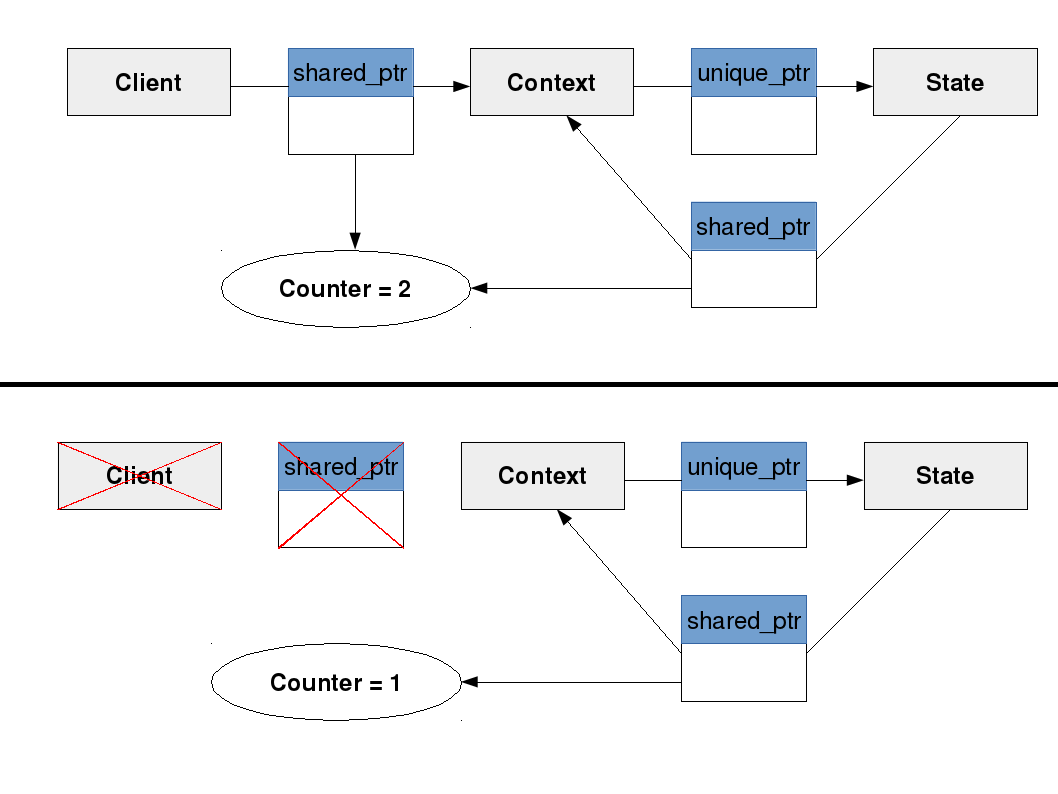
\includegraphics[width=\textwidth]{Images/Shared_ptr_dependency.png}}}
\caption{Shared pointer dependencies}
\label{fig:sharedPointerDependencies}
\end{figure}

\noindent\\ As shown in figure \ref{fig:sharedPointerDependencies} both, \emph{Client} and \emph{State}, refering to \emph{Context} with a shared pointer. \emph{Context} refers to \emph{State} with an unique pointer. If \emph{Client} disappears, the reference counter decreases but does not reach zero because \emph{State} is still refering to \emph{Context}. Therefore \emph{Context} will not be deleted. When \emph{Context} will not be deleted, \emph{State} will also not be deleted because it is still referred by \emph{Context}. A memory leak is the consequence. Deleting the unique pointer, which referes to \emph{State}, manually would solve this problem. Another solution provides the use of weak pointer. 

\begin{figure}[h]{}
\centering
\mbox{\frame{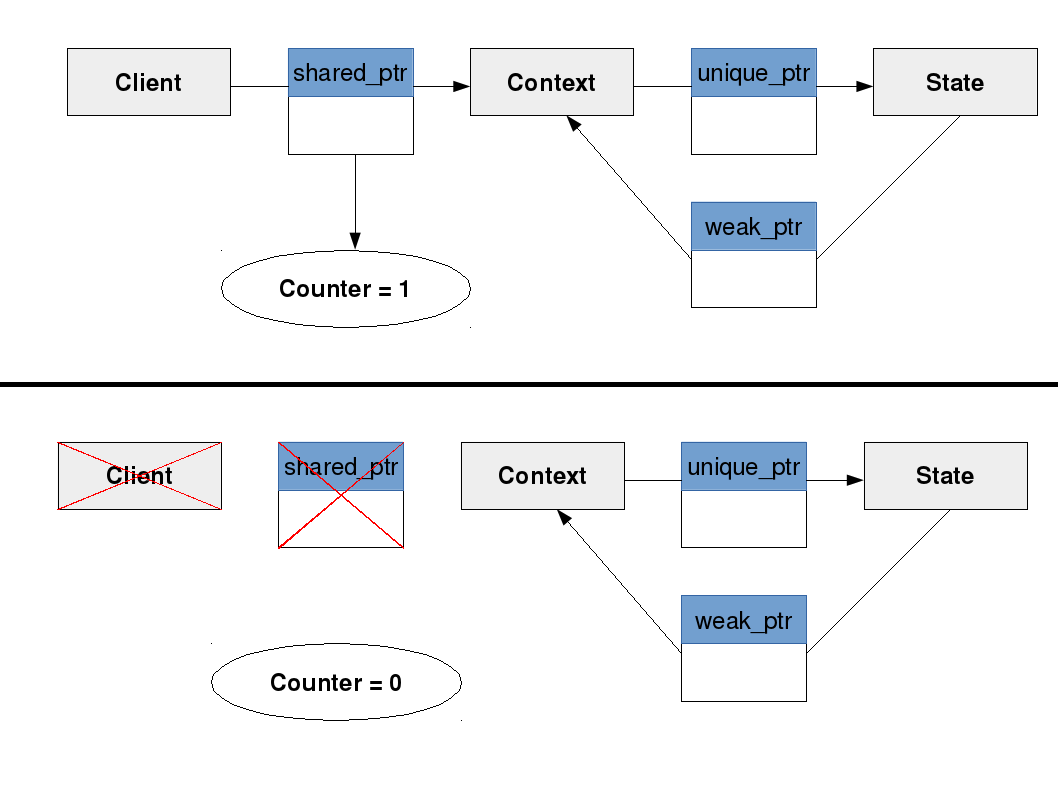
\includegraphics[width=\textwidth]{Images/Weak_ptr_solving_dependency.png}}}
\caption{Weak pointer dependencies}
\label{fig:weakPointerDependencies}
\end{figure}

\noindent Figure \ref{fig:weakPointerDependencies} shows the same example with one difference. Instead of using a shared pointer, \emph{State} only refers to \emph{Context} with a weak pointer. The effect is that the reference counter reaches zero when \emph{Client} disappears because weak pointers have no effect on the reference counter. When the reference counter reaches zero, \emph{Context} will be deleted regardless whether \emph{State} is still refering to \emph{Context}. In this particular example this is no problem because the destructor of \emph{Context} deletes the reference to \emph{State} and \emph{State} will also be deleted. 

\FloatBarrier
\noindent Before calling a member or a function of an object referred by a weak pointer, the software designer must make sure that the weak pointer is pointing to a valid object. For this a weak pointer provides the function \emph{lock}. \emph{lock} casts the weak pointer to a temporary shared pointer which can be used to manipulate the object. (Listing \ref{lst:statePatternLightOffImplementationCpp11}) This temporary shared pointer temporarily increases the reference counter.

\FloatBarrier
\lstinputlisting[caption={State pattern LightOff implementation C++11}\label{lst:statePatternLightOffImplementationCpp11},captionpos=t, backgroundcolor = \color{white}, frame=single, language=C++, firstline=1, lastline=30]{Sourcecode/StatePattern/LightOffCpp11.cpp}

%----------------------------------------------------------------------------------------
%	Bind
%----------------------------------------------------------------------------------------
\subsection{Bind}\label{sec:bind}
 \noindent \emph{bind} is a function which allows to adapt signatures of functions by predefining function parameters. (Listing \ref{lst:bindCpp11})
 
\lstinputlisting[caption={Bind value to function parameter C++11}\label{lst:bindCpp11},captionpos=t, backgroundcolor = \color{white}, frame=single, language=C++, firstline=1, lastline=7]{Sourcecode/bindCpp11.cpp}

\noindent It also provides the option to bind function pointers of memberfunctions to particular instances. \cite[cf.][169 - 172]{Pohmann2013} Line 16 to 21 of listing \ref{lst:statePatternContextCpp11} shows how to use \emph{bind} in combination with \emph{make\_pair} to manage function pointers within a map without using raw pointers. \emph{make\_pair} is a wrapper which combines a key and a value to a map-compatible type. 
 
%----------------------------------------------------------------------------------------
%	Timing for Polymorphism Implementation
%----------------------------------------------------------------------------------------
\subsection{Timing}\label{sec:timingStatePatternPolymorphism}
 
\begin{figure}[h]{}
\centering
\mbox{\frame{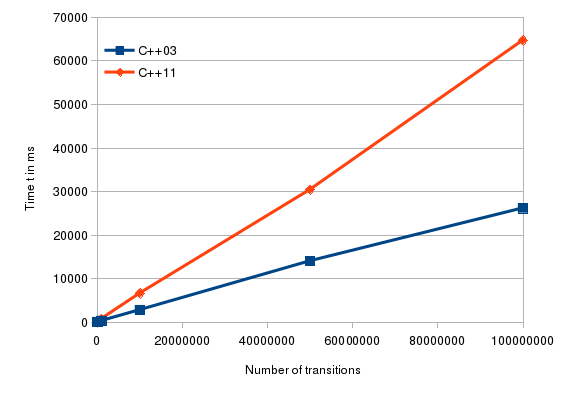
\includegraphics[width=\textwidth]{Images/StatePatternPolymorphismTiming.png}}}
\caption{State pattern polymorphism timing}
\label{fig:statePatternPolymorphismTiming}
\end{figure}

\noindent Figure \ref{fig:statePatternPolymorphismTiming} shows the differences between the C++03 implementation and the C++11 implementation of the state pattern. For changing the state 100,000,000 times, the C++03 implementaton needs about 26 seconds and the C++11 implementation needs about 65 seconds. Table \ref{tab:StatePatternPolymorphismTimingDistributionCpp03} compared with table \ref{tab:StatePatternPolymorphismTimingDistributionCpp11} shows a reduction of the execution time of about 6 seconds for \emph{Context}. The reason for this is the use of an unorderd map with a seek complexity of T(n) = O(1) instead of the use of a normal map with a seek complexity of T(n) = O(log(n)). The dominating factor fo the execution time of the C++11 implementation is caused by the use of smart pointers. With about 35 seconds it is responsible for about 55.2\% of the total execution time.

%Figure \ref{fig:statePatternPolymorphismTiming} shows the differences between the C++03 implementation and the C++11 implementation of the state pattern. For changing the state 100,000,000 times, the C++03 implementation needs about 26 seconds and the C++11 implementation about 65 seconds. %The major factor for this difference is caused by the use of smart pointers instead of raw pointers. Minor differences occur by the use of an unordered map for the dispatcher instead of a normal map. The complexity for finding the requested function pointer within the normal map is T(n) = O(log(n)) where n is the number of available entries. \cite[cf.][]{CppReference2013} As mentioned in chapter \ref{sec:unorderedMap} the complexity of seek time within the unordered map is $\Omega$(1) and in worst case O(n).
 
%\begin{figure}[h]{}
%\centering
%\mbox{\frame{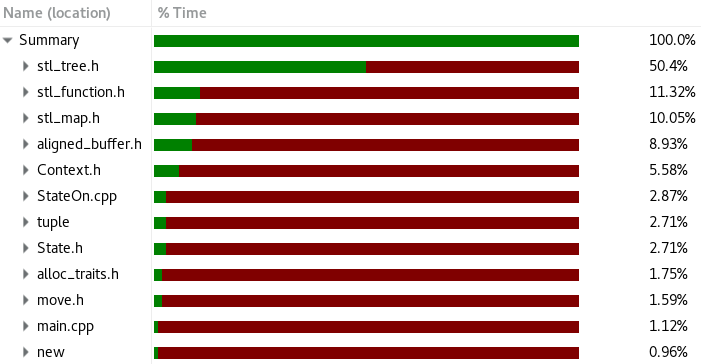
\includegraphics[width=\textwidth]{Images/StatePatternPolymorphismCpp03.png}}}
%\caption{State Pattern polymorphism implementation profiling output C++03}
%\label{fig:statePatternPolymorphismProfilingCpp03}
%\end{figure}

%\FloatBarrier

%\begin{figure}[h]{}
%\centering
%\mbox{\frame{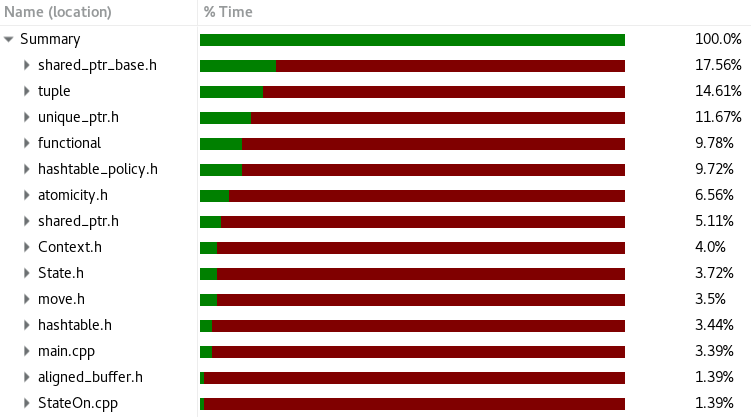
\includegraphics[width=\textwidth]{Images/StatePatternPolymorphismCpp11.png}}}
%\caption{State Pattern polymorphism implementation profiling output C++11}
%\label{fig:statePatternPolymorphismProfilingCpp11}
%\end{figure}
 
\begin{table}[h]\begin{center}
\begin{tabular}{|c|c|c|}\hline
\textbf{Category} & \textbf{Percentage} & \textbf{Time in s}\\
\hline
Context & 93.29 & 24.39\\
\hline
State & 5.58 & 1.45\\
\hline
Main & 1.12 & 0.29\\
\hline
\end{tabular}
\caption{State pattern polymorphism timing distribution C++03}
\label{tab:StatePatternPolymorphismTimingDistributionCpp03}
\end{center}\end{table}
 
\begin{table}[h]\begin{center}
\begin{tabular}{|c|c|c|}\hline
\textbf{Category} & \textbf{Percentage} & \textbf{Time in s}\\
\hline
Context & 28.45 & 18.39\\
\hline
Smart pointer & 55.28 & 35.76\\
\hline
State & 5.11 & 3.30\\
\hline
Main & 1.12 & 0.29\\
\hline
other & 7.79 & 5.03\\
\hline
\end{tabular}
\caption{State pattern polymorphism timing distribution C++11}
\label{tab:StatePatternPolymorphismTimingDistributionCpp11}
\end{center}\end{table}
 
%\noindent the major factor of the execution time of the C++03 implementation is caused by using a map as dispatcher. ( \ref{fig:statePatternPolymorphismProfilingCpp03}) A map uses a binary search tree for managing objects. the seek complexity is O(log(n)). \cite[cf.][821]{Kirch2015} The dominating factor of the execution time of the C++11 implementation is the use of smart pointers. (Figure \ref{fig:statePatternPolymorphismProfilingCpp11}) 'tuple' is used by unique pointers. The second factor of the execution time is the use of the unordered map.
\FloatBarrier

%----------------------------------------------------------------------------------------
%	Memory Consumption for Polymorphism implementation
%----------------------------------------------------------------------------------------
\subsection{Memory Consumption}\label{sec:memoryConsumptionStatePatternPolymorphism}

\noindent For each transition the polymorphism implementation allocates memory for the new state. Figure \ref{fig:polymorphismImplementationMemoryConsumption} shows an allocation of 16 bytes for each transition for the C++03 implementation and 24 bytes for each transition for the C++11 implementation. The overhead of 8 bytes is caused by the use of a weak pointer within state for refering to \emph{Context}. As mentioned in section \ref{sec:smartPointer}, weak pointers also refer to a reference counter. One way to avoid this overhead is to move the weak pointer to \emph{Context} and pass it as function parameter to \emph{State} only when it is needed.  

\begin{figure}[h]{}
\centering
\mbox{\frame{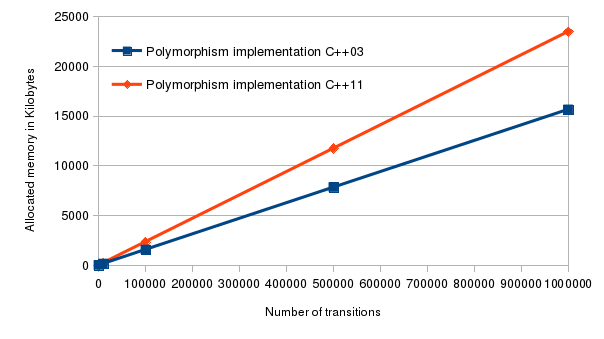
\includegraphics[width=\textwidth]{Images/StatePatternPolymorphismAllocatedBytes.png}}}
\caption{State pattern polymorphism memory consumption}
\label{fig:polymorphismImplementationMemoryConsumption}
\end{figure}

\FloatBarrier
 
%----------------------------------------------------------------------------------------
%	Placement New Implementation
%----------------------------------------------------------------------------------------
\section{Placement new Implementation}\label{sec:placementNewImplementation}
\noindent Dynamic memory allocation is unpredictable. It can take an undefined amount of time for finding a suitable chunk of memory. In worst case no memory is available. Especially for real-time systems the behavior of allocating memory is restricted. One solution C++ provides is the use of the \emph{placement new} operator. The behavior of \emph{placement new} is similar to the \emph{new} operator with the difference that the \emph{placement new} operator takes an already allocated memory address where the new object will be instantiated. (Listing \ref{lst:placementNewCpp11}, line 9)

\lstinputlisting[caption={Placement new operator C++11}\label{lst:placementNewCpp11},captionpos=t, backgroundcolor = \color{white}, frame=single, language=C++, firstline=1, lastline=30]{Sourcecode/StatePattern/LightOffPlacementNewCpp11.cpp}

\FloatBarrier
\noindent In this particular case the combination of smart pointers and the use of the \emph{placement new} operator causes no problems. The change of the object will not be noticed by the smart pointer. However, it is discussable whether the use of the \emph{placement new} operator is still acceptable when the use of the \emph{new} operator is replaced by smart pointers. C++11 does not provide a direct compensation for the \emph{placement new} operator with the same behavior. But with \emph{allocate\_shared} C++11 provides an option to use an own memory management. 

%----------------------------------------------------------------------------------------
%	Allocate_shared
%----------------------------------------------------------------------------------------
\subsection{Allocate\_shared}\label{sec:allocateShared}

The \emph{allocate\_shared} operator is a variant of the \emph{make\_shared} operator. Unlike \emph{make\_shared}, \emph{allocate\_shared} takes an own allocator as parameter for allocating memory. Writing an own allocator which is compliant to the standard allocator is not trivial. Therefore it is recommended to use already existing allocators. Line 40 of listing \ref{lst:statePatternContextPoolAllocatorCpp11} shows the instantiation of a pool allocator with the name \emph{alloc}. In line 15 \emph{alloc} is used for instantiating a new shared pointer refering to an object of class \emph{On}. \emph{alloc} will also be used for transitions within a particular state. (Listing \ref{lst:statePatternLightOffImplementationPoolAllocatorCpp11}, line 8) A pool allocator uses a memory pool with a pre-allocated number of fixed sized memory chunks. (Figure \ref{fig:memoryPool}) If memory is requested, the pool allocator finds the next free memory chunk, and returns the address. In case when a memory chunk is not needed anymore by the requestor, the pool allocator declares this chunk as free to use by other requestors.  

\begin{figure}[h]{}
\centering
\mbox{\frame{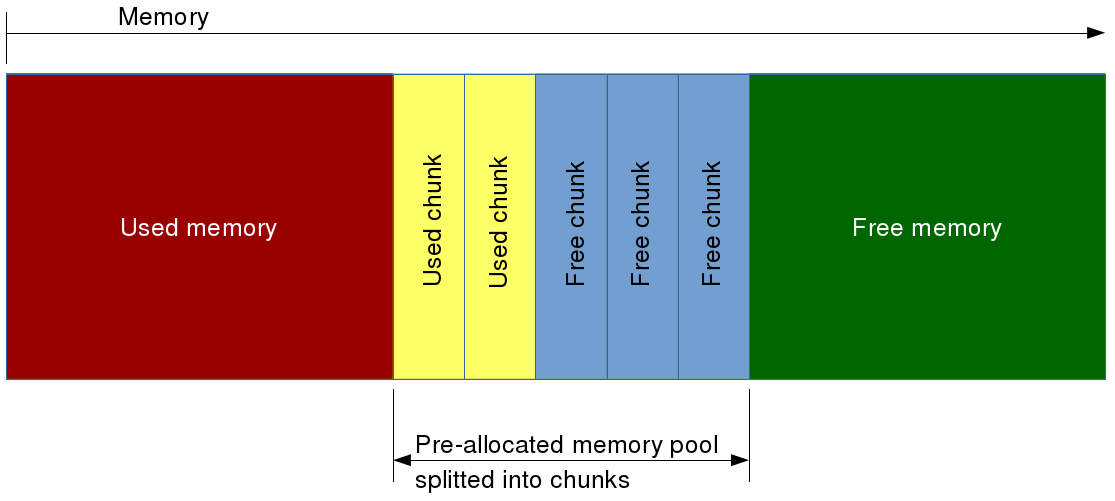
\includegraphics[width=\textwidth]{Images/MemoryPool.png}}}
\caption{Memory pool}
\label{fig:memoryPool}
\end{figure}

\FloatBarrier

\lstinputlisting[caption={State pattern pool allocator Context C++11}\label{lst:statePatternContextPoolAllocatorCpp11},captionpos=t, backgroundcolor = \color{white}, frame=single, language=C++, firstline=1, lastline=43]{Sourcecode/StatePattern/ContextPoolAllocatorCpp11.h}

\lstinputlisting[caption={State pattern pool allocator LightOff implementation C++11}\label{lst:statePatternLightOffImplementationPoolAllocatorCpp11},captionpos=t, backgroundcolor = \color{white}, frame=single, language=C++, firstline=1, lastline=28]{Sourcecode/StatePattern/LightOffPoolAllocatorCpp11.cpp}

%----------------------------------------------------------------------------------------
%	Timing for Placement New implementation
%----------------------------------------------------------------------------------------
\subsection{Timing}\label{sec:timingStatePatternPlacementNew}

\begin{figure}[h]{}
\centering
\mbox{\frame{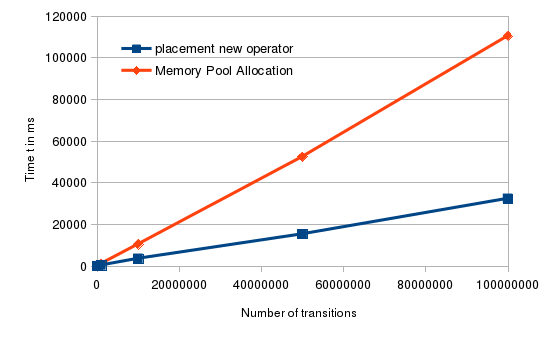
\includegraphics[width=\textwidth]{Images/StatePatternPlacementNewTiming.png}}}
\caption{State pattern placement new timing}
\label{fig:stateMachinePlacementNewTiming}
\end{figure}

\noindent Using \emph{allocate\_shared} including an own memory management is more expensive in timing than using the \emph{placement new} operator. Figure \ref{fig:stateMachinePlacementNewTiming} shows the differences in timing between the \emph{placement new} implementation and the \emph{allocate\_shared} implementation. For changing the state 100,000,000 times, the \emph{placement new} implementation needs about 32 seconds and the \emph{allocate\_shared} implementation needs about 110 seconds. The comparison of profiling output of the \emph{placement new} implementation (Table \ref{tab:StatePatternPlacementNewTimingDistributionCpp11}) with the profiling output of the C++11 polymorphism implementations (Table \ref{tab:StatePatternPolymorphismTimingDistributionCpp11}) shows a reduction of the execution time for smart pointers. The \emph{placement new} operator does not instantiate a new smart pointer. It just instantiates a new refered object on the same memory address where the already existing smart pointer is refering to. This causes a reduction of about 24 seconds for changing the state 100,000,000 times. 

\begin{table}[h]\begin{center}
\begin{tabular}{|c|c|c|}\hline
\textbf{Category} & \textbf{Percentage} & \textbf{Time in s}\\
\hline
Context & 39.34 & 12.73\\
\hline
Smart pointer & 35.92 & 11.62\\
\hline
State & 6.57 & 2.12\\
\hline
Main & 6.21 & 2.01\\
\hline
other & 11.95 & 3.86\\
\hline
\end{tabular}
\caption{State pattern placement new timing distribution C++11}
\label{tab:StatePatternPlacementNewTimingDistributionCpp11}
\end{center}\end{table}

\noindent For every transition the \emph{allocate\_shared} implementation creates a new smart pointer. With 37,8\% of the total execution time the use of \emph{allocate\_shared} is responsible for about 41 seconds. (Table \ref{tab:StatePatternPlacementNewTimingDistributionCpp11}) In addition to that, the used memory pool contributes to the execution time with about 23 seconds. 

\begin{table}[h]\begin{center}
\begin{tabular}{|c|c|c|}\hline
\textbf{Category} & \textbf{Percentage} & \textbf{Time in s}\\
\hline
Context & 20.55 & 22.69\\
\hline
Memory pool & 21.55 & 23.79\\
\hline
Smart pointer & 37.83 & 41.77\\
\hline
State & 4.20 & 4.63\\
\hline
Main & 1.52 & 1.67\\
\hline
other & 14.32 & 15.81\\
\hline
\end{tabular}
\caption{State pattern pool allocator timing distribution C++11}
\label{tab:StatePatternPoolAllocatorTimingDistributionCpp11}
\end{center}\end{table}
\FloatBarrier

%----------------------------------------------------------------------------------------
%	Memory Consumption for Placement New implementation
%----------------------------------------------------------------------------------------
\subsection{Memory Consumption}\label{sec:memoryConsumptionStatePatternPlacementNew}

\noindent Both, the \emph{placement new} implementation and the \emph{allocate\_shared} implementation, have the advantage that transitions cause no memory allocation. Figure \ref{fig:placementNewImplementationMemoryConsumption} shows a constant memory consumption independent of the number of transitions. Because of the memory pool, which allocates a number of memory chunks, the \emph{allocate\_shared} implementation has a slightly higher memory consumption than the \emph{placement new} implementation. This overhead is dependent on the choice of the allocator. The choosen allocator of listing \ref{lst:statePatternContextPoolAllocatorCpp11} does not provide the option to declare the number of pre-allocated chunks. For the state pattern only two chunks are needed. 
 
\begin{figure}[h]{}
\centering
\mbox{\frame{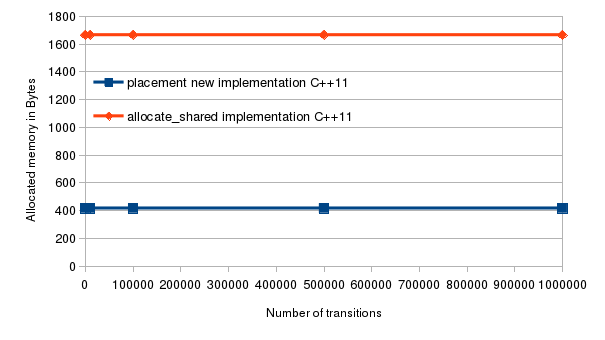
\includegraphics[width=\textwidth]{Images/StatePatternPlacementNewAllocatedBytes.png}}}
\caption{State pattern placement new memory consumption}
\label{fig:placementNewImplementationMemoryConsumption}
\end{figure}

\FloatBarrier



\endgroup}
